\section{INTRODUÇÃO}

A categoria IEEE \textit{Very Small Size Soccer} (VSSS), é uma competição robótica de futebol entre duas equipes de três robôs de dimensões de até 7,5x7,5x7,5cm. 
A competição ocorre dentro de um campo fabricado com uma chapa plana e rígida com dimensões de 150x130cm, na cor preta. Esse campo é delimitado por paredes com quatro cantos em forma de triângulos isósceles sólidos de dimensões 7x7cm, de cor branca e parte superior de cor preta. 
O controle dos robôs é feito por um computador, denominado de técnico. Toda estratégia de jogo é controlada de forma autônoma, ou seja, sem intervenção humana. 
Para realizar esse controle é utilizada uma câmera de vídeo fixada a uma altura não inferior a 2 metros de altura do campo. 
A câmera tem a função de fornecer informações visuais de posicionamento tanto dos robôs da equipe quanto dos adversários dentro do campo.
O reconhecimento por visão computacional dos robôs é feito através de \textit{tags}, posicionadas na parte superior do robô. Essas \textit{tags} identificam o robô através do uso de cores para determinar o time ao qual pertencem, sendo possível utilizar as cores amarela ou azul. O uso de um número maior de \textit{tags} é permitido e optativo, contanto que não sejam iguais às cores utilizadas pela equipe adversária, e servem para identificar cada robô separadamente. A Figura \ref{fig:esquematico} exemplifica a organização do campo utilizado na prova.
% O parágrafo abaixo foi reescrito no parágrafo acima. De nada :)
%O reconhecimento por visão computacional dos robôs é feito através de \textit{tags} posicionadas na parte superior do robô, sendo no mínimo a tag de identificação da equipe do robô podendo ser ela na cor amarela ou azul, as demais tags são optativas da equipe para identificar cada robô separadamente, podendo ter qualquer cor exceto a cor da tag de identificação da equipe adversária. Uma ideia do campo da prova é mostrado na Figura \ref{fig:esquematico}.

\begin{figure}[htbp]
\centerline{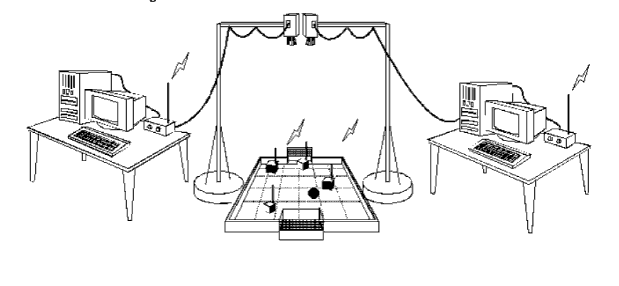
\includegraphics[width=\columnwidth]{capitulos/imagens/Esquematico-de-uma-partida-do-IEEE-VSSS.png}}
\caption{Ambiente da prova}
\label{fig:esquematico}
\end{figure}

Todas as jogadas e estratégias são definidas de forma autônoma pelo técnico, que através dos dados recebidos, envia por meio de uma rádio transmissor qual jogada ou estratégia utilizar durante a jogada para cada robô separadamente.

A equipe TauraBots, fundada no ano de 2015, pelo Professor Dr. Rodrigo da Silva Guerra com o intuito de desenvolver robótica dentro do Centro de Tecnologia (CT) da Universidade Federal de Santa Maria (UFSM), concorrendo principalmente em categorias de robôs humanoides, passando a se envolver recentemente com outras áreas da robótica como carros autônomos e robótica móvel. Participará pela primeira vez este ano na categoria VSSS na presente competição, que vem sendo disputada no Brasil desde o ano de 2003. A equipe que tem como principais conquistas primeiro lugar na RoboCup 2018 na competição de arquearia robotica e terceiro lugar na mesma categoria na AutCup no Irã, terceiro lugar em nos LARC's de 2015 e 2016 na competição Robocup Humanoid League e um terceiro lugar na RoboCar Race no Brasil.

O artigo será dividido em cinco seções. Na seção \ref{construction} será explicado o processo de construção dos robôs e os componentes utilizados, assim como a justificativa de sua escolha.
Na seção \ref{vision} será explicado o sistema de visão utilizado pela equipe. Na seção \ref{strategy} será explicado o sistema de estratégia utilizado na competição. 
Por fim, na seção \ref{conclusion} será apresentada a conclusão do presente artigo.